\documentclass{resume}
\renewcommand{\baselinestretch}{1.1} 

\begin{document}

\fontfamily{ppl}\selectfont

\noindent
\begin{tabular}{lr}  % {\linewidth}{@{}m{0.8\textwidth} m{0.2\textwidth}@{}}
{
    \Large{Foma Shipilov} \\
    \small{
        \clink{
            \href{mailto:foma@shipilov.ru}{foma@shipilov.ru}
            \textbf{$\cdot$} 
            \href{https://t.me/foma2u}{@foma2u}
        } \\
        Moscow, Russia
    }
} & 
{
    \hfill
    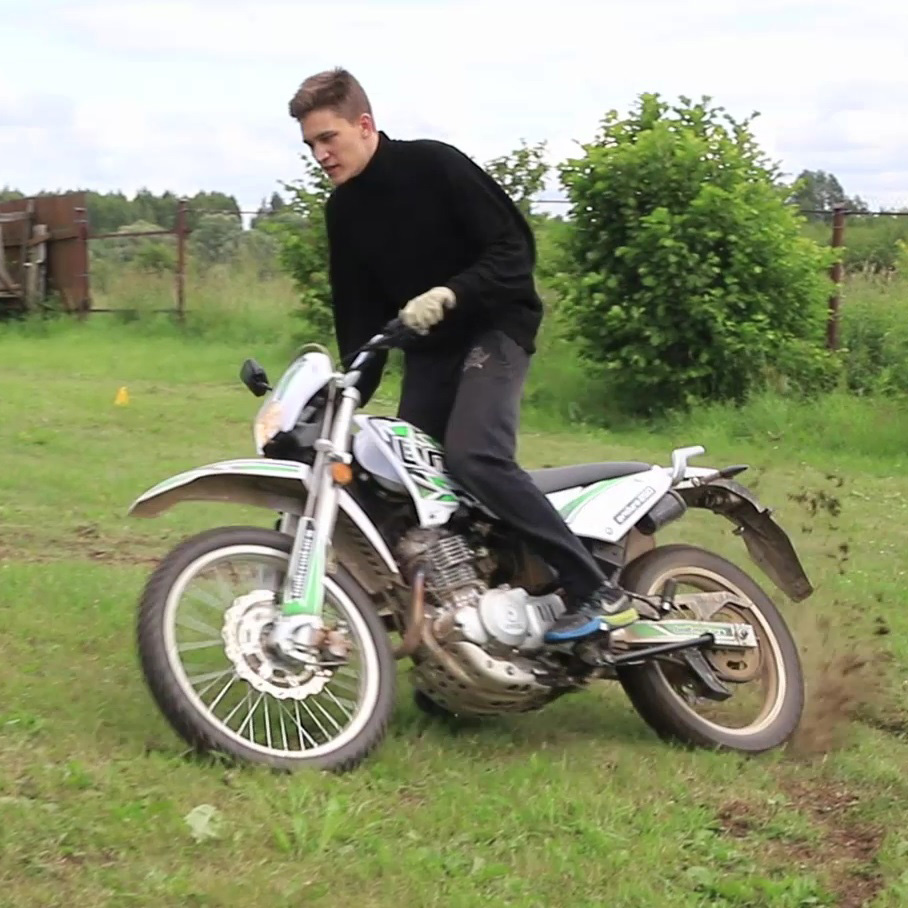
\includegraphics[width=2.8cm]{images/gr.jpg}
}
\end{tabular}
%\vspace*{-1.5em}
\begin{center}
\begin{tabularx}{\linewidth}{@{}*{2}{X}@{}}
% left side %
{
    \csection{EXPERIENCE}{\small
        \begin{itemize}
            \item \frcontent{HSE University}{Intern-researcher @ LAMBDA\\
            Lecturer @ Big Data and Information Retrieval School}{-- Applying deep learning to online filtering and reconstruction of aerogel detectors\\ 
                \href{https://doi.org/10.1134/S106377882305037X}{What Machine Learning Can Do for Focusing Aerogel Detectors, Physics of Atomic Nuclei 86, 864 (2023)}\\
                \href{https://doi.org/10.3103/S0027134924702369}{Machine Learning for FARICH Reconstruction at NICA SPD, MSU Physics Bulletin 79 S2, 906 (2024)}\\
                -- Teaching courses: Deep Learning 1, Introduction to Deep Learning}{November 2021 onwards}
            \item \frcontent{Sber}{Manager @ Anti-Fraud Department\\
                Intern @ Sber AI Lab}{-- Developed an anti-fraud AI solution (joint with HSE)\\
                -- Evaluated Temporal Point Process models on MIMIC-IV medical dataset\\
                \href{https://doi.org/10.1016/j.neucom.2026.132771}{HoTPP benchmark: Are we good at the long horizon events forecasting?, Neurocomputing 672, 132771 (2026)}}{March 2024 -- December 2024}
            \item \frcontent{Huawei}{Assistant Engineer @ Noah’s Ark lab}{-- Remastered TV-series using GANs;\\
                -- Developed non-linear CNN degradation model for super-resolution of real-world images.}{November 2020 -- September 2021}
        \end{itemize}
    }
    \csection{EDUCATION}{\small
        \begin{itemize}
            \item \frcontent{PhD Computer Science, Academic Track}{HSE University}{}{Currently undergoing}
            \item \frcontent{MSc Data Science $\times2$}{HSE University, Skoltech (Studied in English)}{}{2025, Academic Honors Diploma}
            \item \frcontent{BS Computer Science}{HSE University}{}{2023, Academic Honors Diploma}
        \end{itemize}
    }
} 
% end left side %
& 
% right side %
{
    \csection{SKILLS}{\small
        \begin{itemize}
            \item \textbf{ML \& Data Analysis} \\
            {\footnotesize -- Computer vision, super-resolution, GANs, diffusion models, RNNs, transformers, deep learning for audio, deep Bayesian learning, mode connectivity\\
            -- PyTorch, scikit-learn, OpenCV, NumPy, JAX, Polars, PySpark, Hadoop, Vowpal Wabbit}
            \item \textbf{Languages \& Frameworks} \\
            {\footnotesize Python, C, C++, C\#, Haskell, x86/ARM Assembly, HTML/CSS/JS, ReactJS, Lua}
            \item \textbf{CI/CD \& Other} \\
            {\footnotesize Docker, WandB, Hydra, GitHub Actions, QuickCheck, GDB, Arch Linux, Shell, ZFS}
        \end{itemize}
    }
	\csection{AWARDS \& RECOGNITION}{\small
		\begin{itemize}
            \item \frcontent{Yandex Scholarship}{HSE University}{}{2022}
			\item \frcontent{Vysshaya Liga, Math \& Informatics}{HSE University}{Degree I \& III Diploma}{2021, 2022}
			\item \frcontent{Ya Professional, Math Olympiad}{Yandex}{Prize-winner}{2021, 2022}
			% \item \frcontent{``Pokori Vorob'yovi Gori'' Math Olympiad}{Moscow State University}{Winner}{2019}
			%\item \frcontent{Phystech, Math \& Physics Olympiads}{Moscow Institute of Physics and Technology}{Winner}{2019}
		\end{itemize}
	}
    %\csection{OTHER HIGHLIGHTS}{\small
    %    \begin{itemize}
    %        \item {\footnotesize Conducted biology studies within \textit{Structural and Functional Research of G-protein-coupled Cell Surface Receptors Using 3D Modeling} school project.}
    %    \end{itemize}
    %}
    \csection{PROJECTS}{\small
    \begin{itemize}
        \item \frcontent{mars-reproducibility \clink{\href{https://github.com/xiyori/mars-reproducibility}{[github.com]}}}{Reproducing MARS tensor decomposition 2023 paper}{}{PyTorch}
        \item \frcontent{secHNet \clink{\href{https://github.com/xiyori/secHNet}{[github.com]}}}{PyTorch in Haskell from scratch}{}{Haskell, C}
        % \item \frcontent{Visual Turing \clink{\href{https://github.com/xiyori/turing_machine_emulator}{[github.com]}}}{Turing machine IDE in \textit{C++}}{}{}
        %\vspace*{-3em}
    \end{itemize}
    }
    \csection{HOBBIES \& INTERESTS}{\small
        \vspace{0.32cm}
        \begin{tabular}{cccc}
            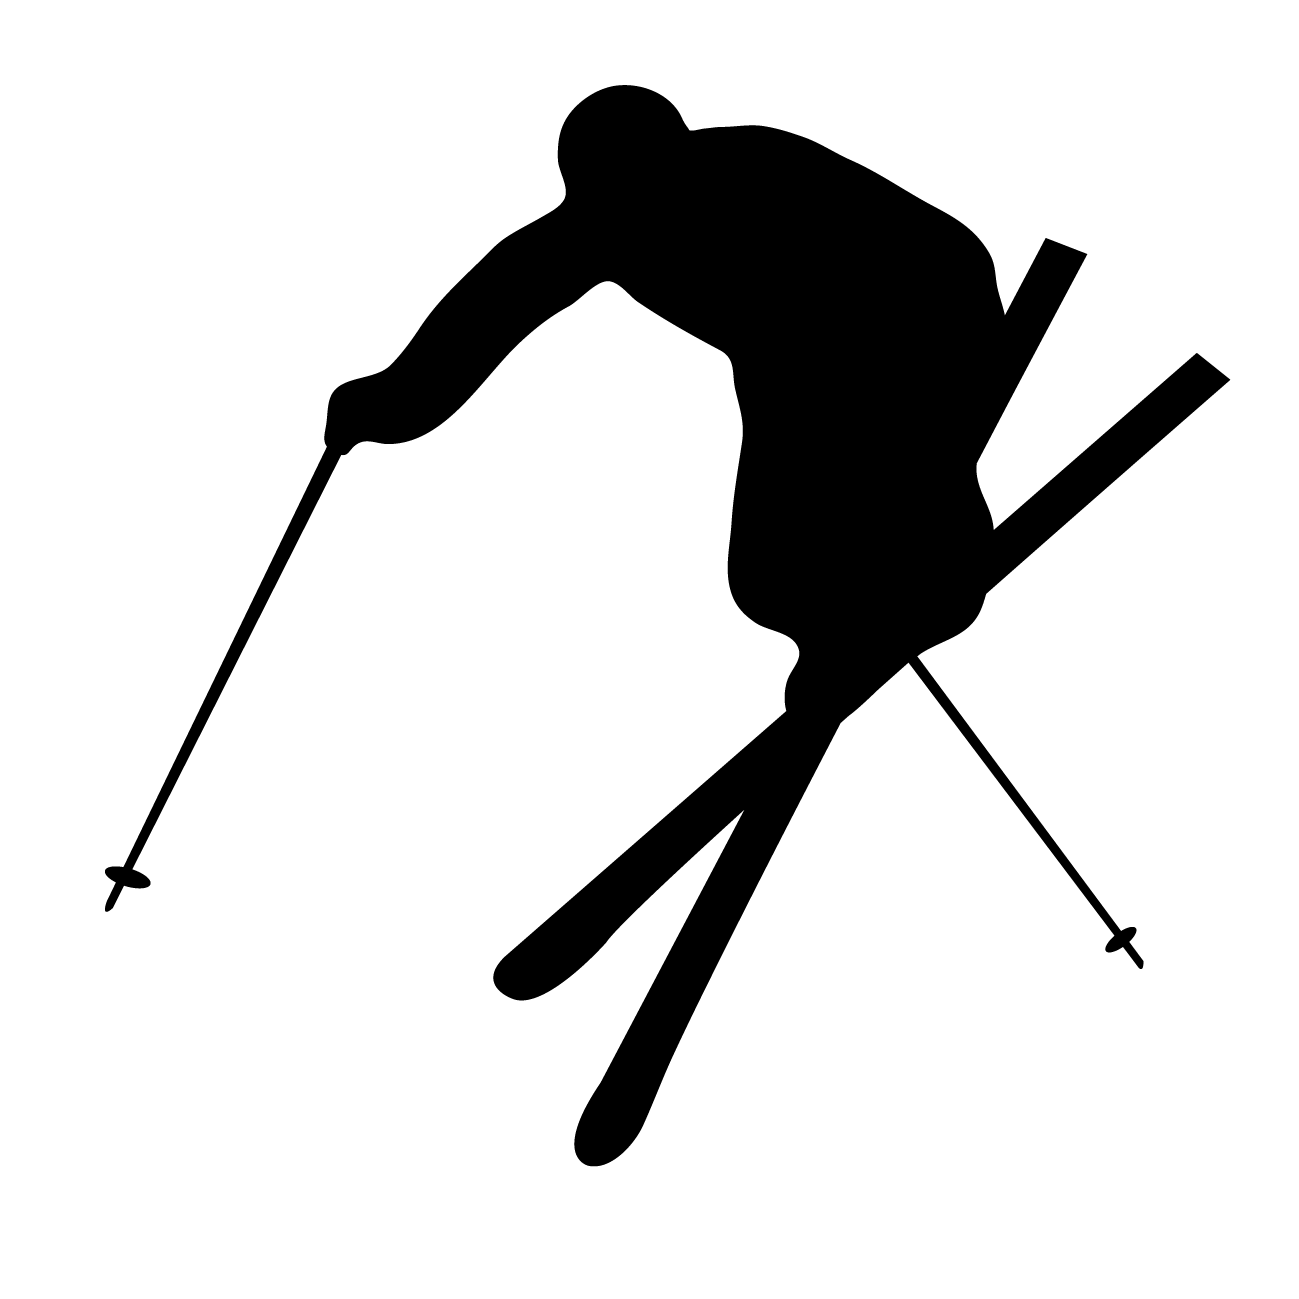
\includegraphics[width=0.8cm]{images/skiing.png} &
            
\includegraphics[width=0.8cm]{images/hyperspeedcube.png} &
            
\includegraphics[width=0.8cm]{images/homelab.png} &
            
\includegraphics[width=0.8cm]{images/headphones.png} \\
            {\footnotesize Alpine skiing} & {\footnotesize Hypercubing} & {\footnotesize Homelab} & {\footnotesize HRTF measurements}
        \end{tabular}
    }
}
\end{tabularx}
\end{center}
\end{document}
